The dataset is large and noisy. A model is needful to guide the data analysis and to give an interpretation to all results.

The guiding idea of the Minimal Effort model is that inheritance is designed to better promote code reuse and, in this sense, to minimize the effort in writing programs.

The model is a mean field approximation for graphs and it allows you to obtain some interesting features, useful in all next chapters. 

%******************************************************************************************************************************
\section{Reuse and Effort}
Programs are created to perform tasks and solve problems and, in object-oriented programming, each task is performed with modular code, the objects, often organized in hierarchies.

In a first approach, let's suppose that only terminal nodes of inheritance graphs compose the effective solution of the problem, while all nodes at higher levels are made for code reuse purposes only.

Terminal nodes are the leaves of the tree which represents the hierarchy. Leaves are given by the problem, but rules are needed in order to build the whole tree from its leaves. How can we group leaves in different levels? Which principle may guide us?

\subsection{Why use inheritance?}
Assuming that inheritance most important effect in graph structure is code reuse, we can start from the $\enne$ classes which represent the solution of the problem.

Suppose that the implementation of two of this classes is very similar. Then you can move mutual code lines in a third node, in the upper level of this tree.

In this way, one can avoid writing twice the mutual lines, creating a node which shares its lines with the two leaves. In this sense, we are guided by a minimum effort principle. Obviously, one can group more than two nodes and try to absorball mutual lines of leaves code in higher level.

The function effort $\Ee$ of a tree is defined simple as
\[ \Ee = \sum_{\sigma}^{\enne} \text{cost}(\sigma) \]
a sum over all nodes, were each node cost is normalized as
\[ \text{cost}(\sigma) = 1 - \varepsilon \]
were $\varepsilon$ represent the fraction of code which inheritance permits you to save.

\subsection{Competition}
The trivial minimum is reached when all leaves can share all its code in one upper node, and so when all leaves are identical. To avoid triviality we need a contrasting mechanism: competition arise from the fact that leaves are different in its implementation and more are the classes that one is trying to group together and less is the number of code lines that can be shared, and so $\varepsilon = \varepsilon (\emme)$.

To find an explicit form for $\varepsilon (\emme)$, consider each class made of an unordered sequence of $\kappa$ symbols. The number of available symbols is $\Esse$ and symbols are equally likely. Symbols that compose classes represent functions, or private variables, or something that can be considered a unit for the code at this abstracted level.

How much code can be shared by $\emme$ nodes? The probability to draw a selected symbol in a sequence of trials with replacement is given by the Binomial distribution of parameters $p = \frac{1}{\Esse}$ and $\kappa$ as the number of trials. We can calculate the probability to find the selected symbol once or more as 1 less the probability to not find the selected symbol, and so
\[ p = 1 - \left ( 1 -\frac{1}{\Esse} \right )^\kappa \]
Now suppose $\Esse \to \infty$ and $\kappa \to \infty$ and define $\beta$ as
\[ \beta= \frac{\kappa}{\Esse} \]

In this limit, we can expand
\[ e^{-\beta}= \lim_{\Esse \to +\infty} \left( 1 - \frac{1}{\Esse} \right)^{\beta \Esse} \]
and then we can rewrite the probability to find a selected symbol in a sequence of extractions as
\[ p = 1 - e^{-\beta} \]
Consider $\emme$ indipendent sets of $\kappa$ extractions. The probability to find the selected symbol in all $\emme$ sets is simply 
\[ \rho = \left(1 - e^{-\beta}\right)^{\emme} \]

We are interesting in the fraction of code $\varepsilon (\emme)$ that $\emme$ nodes can share. Since all symbols are equal for our groupment, we can multiply the last result by $\Esse$, and divided it by the length of the sequence $\kappa$ to normalize the result.
\[ \varepsilon (\emme) = \frac{\Esse}{\kappa} \left(1 - e^{-\beta}\right)^{\emme} = \frac{1}{\beta} \left(1 - e^{-\beta}\right)^{\emme} \equiv e^{-\alpha \emme}\]

It is now possible to evaluate the cost of each single node and then of each graph.
\[ \text{cost}(\sigma) = 1 - e^{-\alpha \emme} \]
\begin{figure}[ht]%
\center
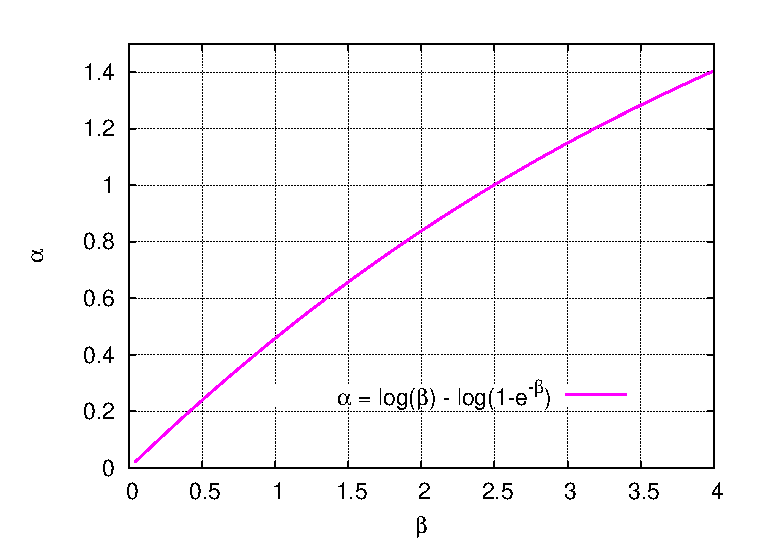
\includegraphics[width=9cm,draft=false]{grafici/alphabeta.eps}
\caption{\label{alphabeta} \footnotesize\textbf{$\boldsymbol{\alpha}$ and $\boldsymbol{\beta}$} - $\alpha$ is small for small $\beta$, and viceversa. }
\end{figure}

\newpage
\vphantom{ciao}
\vspace{5cm}
\begin{figure}[H]%
\center
%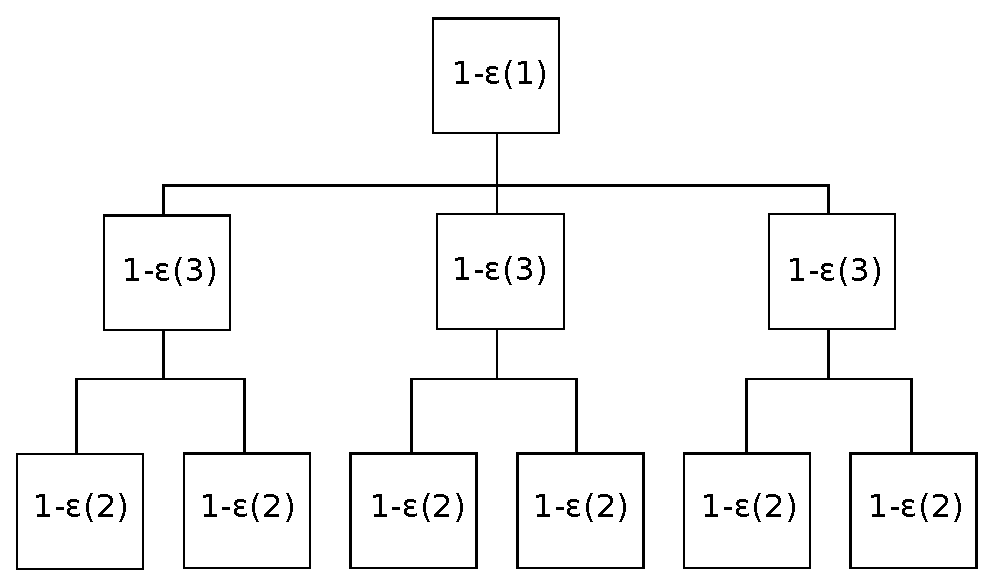
\includegraphics[width=\textwidth,draft=false]{images/effort.eps}
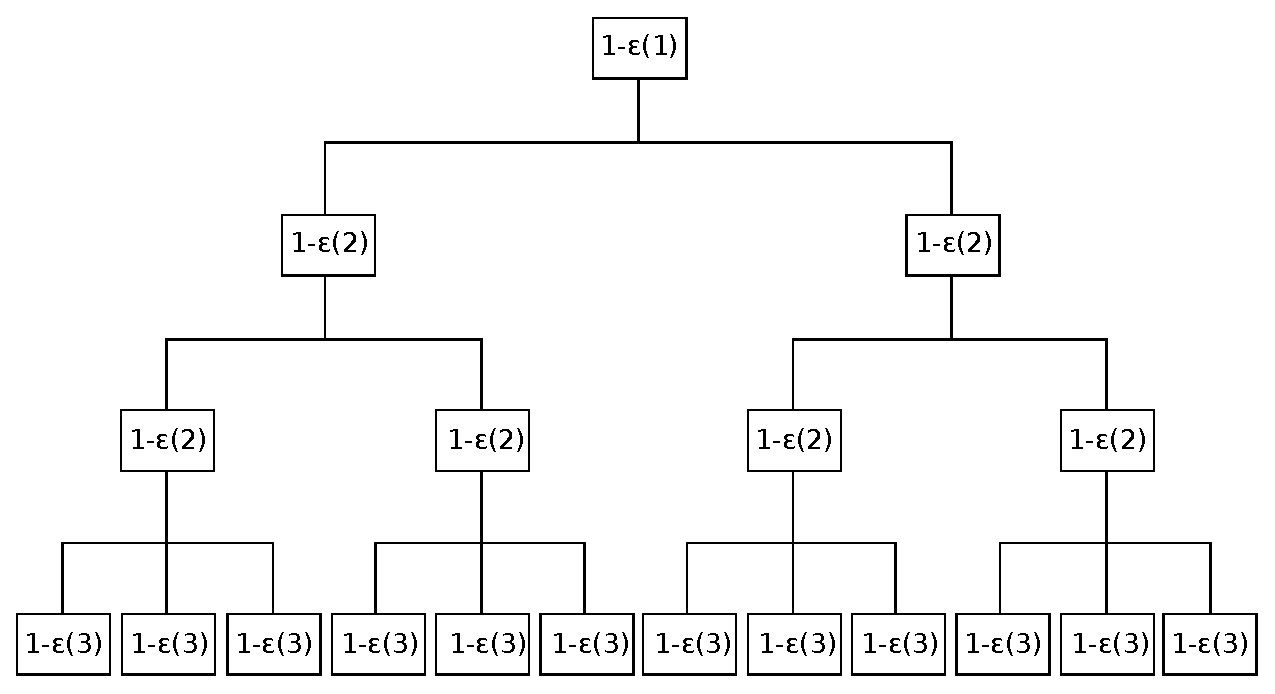
\includegraphics[width=\textwidth,draft=false]{images/effort2.eps}
\caption{\label{effort} \footnotesize\textbf{Mean field tree} - The Minimal Effort model estimates the effort necessary to build a graph as the sum of the cost of each node. }
\end{figure}
\newpage


\subsection{Minimizing the effort}
Despite the simplicity of the functional $\Ee$, it's not easy to make calculation keeping the whole complex structure of all possible trees. We need to simplify the topology.

Levels are labeled $\elle$, where the level $\elle=0$ correspond to the set of leaves and the level $\elle=\Elle$ is the set containing the root only. 
At each level $\elle$, the tree is essentially a set of nodes $\enne(\elle)$.

We can estimate the mean number of brothers that each node may have. It is given by the number of nodes at a level $\enne(\elle)$ divided by number of available parents, and so the number of nodes at successive level $\enne(\elle+1)$
\[ \emme(\elle) = \frac{\enne(\elle)}{\enne(\elle+1)} \]

Forgetting all details, let's consider a tree configuration all expressed by the number of nodes at each level, ignoring which nodes are linked together and which are not.
\[ \{ \enne(\elle) \}_{\elle=0}^{\Elle} = \{ \enne(0), \enne(1), \dots, \enne(\Elle)\equiv 1\} \]

With this simplification we can rewrite the effort as a sum over levels, and then
\[ \Ee [\Elle,\{ \enne(\elle) \}] = \sum_{\elle=0}^{\Elle-1} \left [ 1 - \varepsilon \left ( \frac{\enne(\elle)}{\enne(\elle+1)} \right ) \right ] \enne(\elle) \]
And expliciting the function $\varepsilon$ we obtain
\begin{equation}
\label{functional}
\Ee [\Elle,\{ \enne(\elle) \}] = \sum_{\elle=0}^{\Elle-1} \left ( 1 - e^{- \alpha \frac{\enne(\elle)}{\enne(\elle+1)}} \right ) \enne(\elle)
\end{equation}
 
It is now possible to obtain the minimum of the Effort $\Ee$ respect to the total number of levels $\Elle$ and the number of nodes at each level $\enne(\elle)$.
\[ \Ee^* = \min_{\Elle \, \{ \enne(\elle) \}} \Ee [\Elle,\{ \enne(\elle) \}]  \]

%------------------------%
\section{Numerical solutions}
Despite the lack of details about tree shapes, the model allows you the study of some important quantities, like nodes mean degree or population at each level. In this section results of numerical simulations about this quantities are shown for different parameters.

The minimization of the Effort functional \eqref{functional} has been made with the interior point method implemented in the program Wolfram Mathematica \cite{math}. The number of nodes, which is a discrete quantity by definition, is allowed to be real numbers in minimization process.

%---
\subsection{Finding optimal depth}
The Effort $\Ee$ is minimized respect to the number of nodes at each level $\{ \enne(\elle) \}$ and the depth $\Elle$, which is the maximum level accessible by the tree, that is populated by only one node, the root.

Free parameters of the model are $\enne(0)$, which is defined by the number of leaves, or the number of nodes necessary to solve the problem for which the tree has been created, and $\alpha$ which represents the abstractability.

Fixing reasonably values for these parameters, as $\enne(0)=1000$ and $\alpha=0.1$, we can look for the optimal depth $\Elle^*$ which minimize $\Ee$.
%
\begin{figure}[ht]%
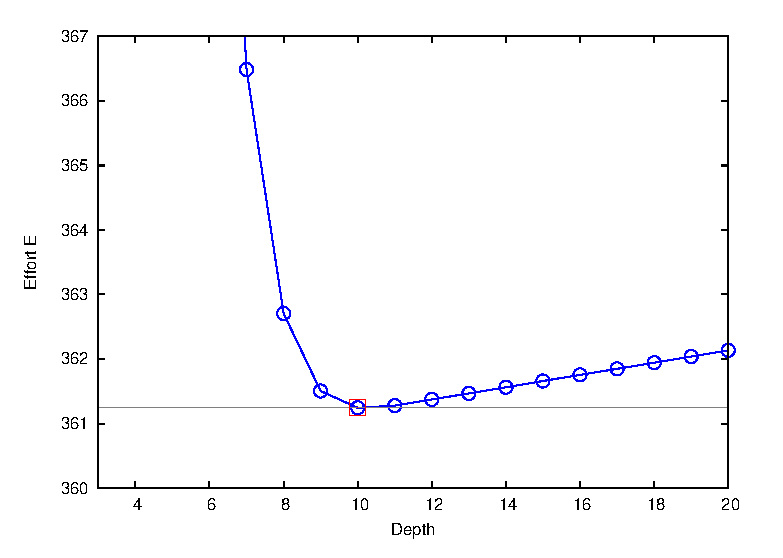
\includegraphics[width=\textwidth,draft=false]{grafici/effVSdepth.1000.1.eps}
\caption{\label{FeffVSdepth} \footnotesize\textbf{The Effort as a function of depth} - When $\alpha=0.1$ and $\enne(0)=1000$, simulations show that the Effort is minimal for $\Elle=10$.}
\end{figure}

The numerical solution leads to $\Elle^*=10$, as showed in figure \ref{FeffVSdepth}.

%--
\subsubsection{Population at each level}
When the depth is optimal, the number of nodes is exponential in its dependence from the level, as shown in figure \ref{FpopVSlevdepth}.

Starting from a depth value lower than the optimal one and increasing it, the function representing the population at each level increases, approaching gradually the exponential function.

When optimal tree is reached, a further depth increase is ineffective to modify significantly the Effort value. The tree structure changes with the depth increase, but only near the optimal depth. When this point is exceeded of two units, the tree structure remains substantially unchanged and the only effect of depth increase is the addition of a node at the top of the graph, and so the addition of a new root linked to the old one only.

%--
\subsubsection{Outdegree mean}
Simulations of the function $\emme(\elle)$ reveal the behavioral change in population distribution respect to fixed depth. 

The ratio between the number of nodes of two consecutive levels is always increasing with levels until the optimal depth is reached. Then this quantity tends to be decreasing with levels, as shown in figure \ref{FpopVSlevdepth}.

This behavior is telling us that the effort is minimized when the outdegree mean is substantially constant with levels.

While number of nodes are allowed to be real number, levels are discrete quantities. We can then suppose that the minimum of functional $\Ee$ is somewhere between $\Elle =10$ and $\Elle =11$.

\begin{figure}[p]%
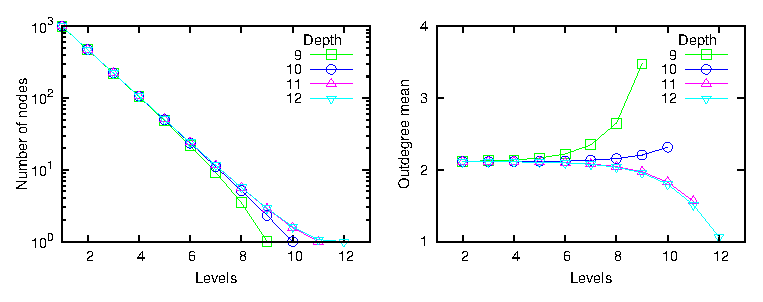
\includegraphics[width=\textwidth,draft=false]{grafici/Mdepth.eps}
\caption{\label{FpopVSlevdepth} \footnotesize\textbf{Distribution of nodes and outdegree mean for different values of depth} - When the depth is optimal, $\Elle=10$, nodes distribution is exponential, as showed in the left hand side figure. The right hand side shows that the optimal depth is the one for which outdegree vary as less as possible with levels. The costant function is often non accessible due to the fact that levels are discretized.}
\vspace{1cm}
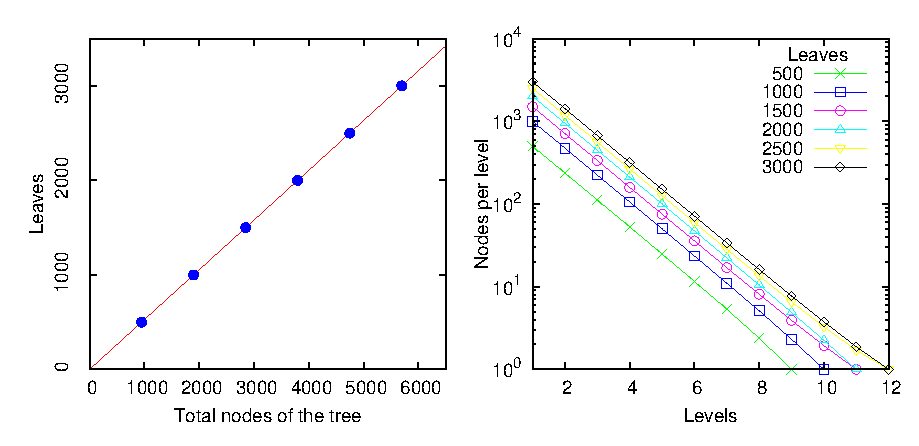
\includegraphics[width=\textwidth,draft=false]{grafici/Mnodes.eps}%$y(x) = x*0.526328(+/- 0.0002096) + 2.10748 (+/- 0.7746)$
\caption{\label{FleaVSnod} \footnotesize\textbf{Leaves and nodes of optimal trees} - The figure on the left hand side shows that the dependence between total nodes and fixed initial leaves is linear. The linear fit leads to $y(x) \sim x/2 + 2$. At the right hand side, populations of nodes at each level of optimal depth for different values of leaves.}
\end{figure}

%---
\subsection{Varying number of leaves}
In order to complete this analysis, we have to study how results change varying the fixed initial parameters.  In this section, the abstractability is fixed $\alpha=0.1$.

The parameter $\enne(0)$ is the one which governs the total number of nodes of the tree. The dependence between nodes and leaves is linear, while the number of nodes is an exponential function of nodes for optimal trees, as showed in \ref{FleaVSnod}. There is a small deviation caused by the discrete nature of levels, that is visible when the level approaches the root.

The optimal depth, the one which minimizes the Effort, moves with the number of leaves. The minimum grows while the number of leaves $\enne(0)$ grows too. The dependence is almost linear, discretized by levels, as showed in \ref{FeffVSdepleaves} at the left hand side.

Keeping $\alpha=0.1$ fixed, and moving the number of leaves, we can observe the particular behavior of the outdegree mean as a function of levels showed at the right hand side of figure \ref{FeffVSdepleaves}. The optimal tree is the one whose outdegree mean is constant respect to levels. When the constant function is not accessible, the nearest function is chosen as optimal. This is the reason for which the derivative of outdegree respect to levels is oscillatory as a function of number of leaves.
\begin{figure}[p]%
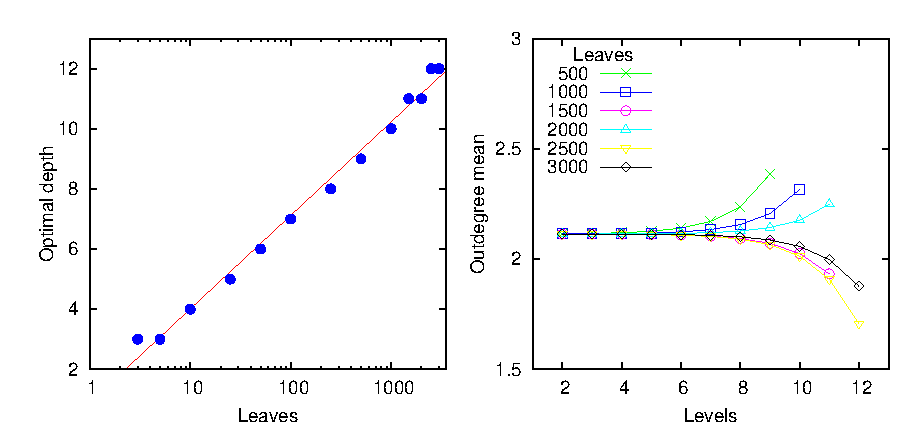
\includegraphics[width=\textwidth,draft=false]{grafici/Mvarleaves.eps}
\caption{\label{FeffVSdepleaves} \footnotesize\textbf{Optimal depth and outdegree mean for different values of leaves} - The optimal depth increases with the number of leaves as $y(x) \sim x/1000 + 9$. At the right hand side, the outdegree mean as a function of levels for optimal depth.}
\vspace{1cm}
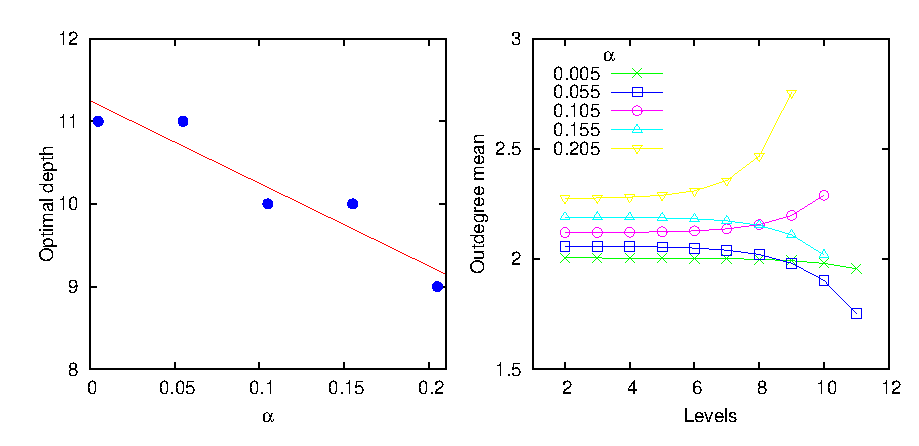
\includegraphics[width=\textwidth,draft=false]{grafici/Mvaralpha.eps}
\caption{\label{FeffVSdepalpha} \footnotesize\textbf{Optimal depth and outdegree mean for different values of $\boldsymbol{\alpha}$} - The optimal depth decreases with the number of leaves as $y(x) \sim 11 - 10x$. At the right hand side, the outdegree mean as a function of levels for optimal depth.}
\end{figure}

%---
\subsection{Varying abstractability $\alpha$}
The parameter $\alpha$ quantifies the portion of code that can be abstracted in higher levels, and so it represents the number of lines that nodes hold in common. In this section, the number of leaves is fixed $\enne(0)=1000$.

Numerical simulations show that if $\alpha$ is high, the optimal depth is low and vice versa. The position of the minimal Effort respect to depth moves linearly with $\alpha$, as showed in the left hand side of figure \ref{FeffVSdepalpha}.

The outdegree mean increses with $\alpha$, while its derivative remains oscillatory due to discrete levels. See figure \ref{FeffVSdepalpha}.
%


